\section{Base de datos de artículos}
La base de datos utilizada para realizar los experimentos computacionales de lo propuesto en este trabajo es la proporcionada por el artículo \textit{\textquotedblleft A Data-Driven Journey through Software Engineering Research\textquotedblright}\cite{dataDrive}. La misma contiene artículos relacionados con la ingeniería de software presentados en diferentes conferencias entre los años 1975 y 2011 catalogados por autores, tópicos, venues y afiliaciones. La decisión de utilizar esta base de datos es por la completitud de la información y que al contener una gran cantidad de elementos requiere de algoritmos eficientes. La base de datos contiene cerca de $7800$ artículos de los que se tiene los autores, la conferencia en que fueron presentados y se encuentran clasificados en tópicos. Esta clasificación, conocida como \texttt{topicProfile}, se expresa en porcentajes para cada uno de los tópicos que son tratados. De los $9800$ autores se tiene la información de la universidad a la que pertenecen y de las universidades en que región se encuentran.\\
El \texttt{topicProfile} es lo que permitirá definir la similitud, no sólo entre los artículos, sino también entre los autores y las universidades de la base da datos de una manera prácticamente directa.\\

Los criterios de las búsquedas realizadas sobre la base de datos se concibieron a partir de lo que se considera que es de interés general. Por ejemplo, quiénes son los autores que escribieron artículos similares de distintas universidades o las universidades de diferentes regiones donde se escribieron artículos de los mismos tópicos.\\
Por lo establecido en \cite{compositeRetrival} para las búsquedas se deben realizar las siguientes definiciones:
\begin{itemize}
  \item \textbf{Similitud}: Función que dado dos ítems devuelve la similitud entre estos.
  \item \textbf{Costo}: Función que dado un ítem devuelve el costo del mismo.
  \item \textbf{Presupuesto}: El presupuesto que se tiene, el cual no podrá ser excedido por ningún bundle.
  \item \textbf{Complementariedad}: Propiedad del ítem que es único en cada bundle.
\end{itemize}

Para todas las búsquedas, sin importar el ítem que sea (artículo, autor o universidad), se definió que el costo de cada ítem sea de una unidad y que el presupuesto para cada búsqueda es de cinco unidades. En consecuencia, todos los bundles de todos los resultados contienen como máximo cinco ítems. Se decidió así porque no tiene sentido asociarle un costo a los artículos, autores, universidades y solo nos interesa que el bundle tengo como máximo un número fijo de elementos. Además se decidió que sean diez los bundles devueltos en cada búsqueda. El motivo para tomar esta decisión es que un humano pueda valorizar el resultado propuesto fácilmente. Entonces, de aquí en adelante, para cada criterio de búsqueda se deben definir únicamente la función de similitud y la propiedad de complementariedad.\\

Como se mencionó anteriormente, en la base de datos cada artículo cuenta con su \texttt{Topic Profile}. El \texttt{Topic Profile} define el perfil de cada artículo asignándole un porcentaje a cada tópico que se hace referencia. En el caso del artículo \texttt{A Cognitive-Based Mechanism for Constructing Software Inspection Teams} el \texttt{Topic Profile} se compone por los tópicos  REQUIREMENTS, RELIABILITY, TESTING y SOFTWARE QUALITY. El porcentaje de cada uno de estos es 71.43 \%, 17.86 \%, 7.14 \% y 3.57 \% respectivamente.\\

El modelo computacional del perfil de cada artículo es un vector de $n$ dimensiones, dónde $n$ es la cantidad de tópicos y cada posición representa un tópico diferente. El valor de cada posición del vector es el porcentaje del tópico que le corresponde a ese artículo según el \textit{Topic Profile} de la base de datos. Más adelante se explica como estos vectores se utilizan para comparar la similitud entre los artículos.\\

Para los autores no se cuenta con información más allá de los artículos que escribieron, pero sólo con eso alcanza para poder generar un perfil de autores, por lo tanto para cada autor se hace la suma vectorial de cada uno de los \texttt{Topic Profile} de los artículos en los cuales participó y con eso se obtiene el \texttt{Topic Profile de Autores}.Para obtener el perfil de las universidades se aplicó el mismo criterio que para los autores, de hacer la suma vectorial de cada uno de los \texttt{Topic Profile de Autores} pertenecientes a la misma universidad y así generar el \texttt{Topic Profile de Universidades}. En ambos casos se aplica la normalización sobre los vectores resultantes.

Ejemplo de los perfiles de los elementos:

\begin{description}
 \item[Artículo - Topic Profile - Autores]
 \item Artículo 1 - $[$0.20, 0.40, 0.40, 0.00$]$ - Autor 1, Autor 2, Autor 3
 \item Artículo 2 - $[$0.30, 0.70, 0.00, 0.00$]$ - Autor 2, Autor 3
 \item Artículo 3 - $[$0.00, 0.10, 0.00, 0.90$]$ - Autor 2
 \item Artículo 4 - $[$0.00, 0.00, 1.00, 0.00$]$ - Autor 1, Autor 3
\end{description}

\begin{description}
 \item[Autor - Topic Profile - Universidad]
 \item Autor 1 - $[$0.14, 0.27, 0.95, 0.00$]$ - Universidad 1
 \item Autor 2 - $[$0.30, 0.74, 0.25, 0.55$]$ - Universidad 2
 \item Autor 3 - $[$0.27, 0.60, 0.76, 0.0$]$ - Universidad 2
\end{description}

\begin{description}
 \item[Universidad - Topic Profile]
 \item Universidad 1 - $[$0.14, 0.27, 0.95, 0.00$]$
 \item Universidad 2 - $[$0.31, 0.72, 0.54, 0.30$]$
\end{description}

Las consultas realizadas son:
\begin{enumerate}
	\item
		Artículos con tópicos similares presentados en distintas conferencias.
		\begin{itemize}
			\item \textbf{Similitud}: Función que compara el perfil de cada artículo.
			\item \textbf{Complementariedad}: Lugar dónde fue presentado.
		\end{itemize}

	\item
	Autores que escribieron artículos con tópicos similares afiliados en universidades distintas.
	\begin{itemize}
		\item \textbf{Similitud}: Función que compara el perfil de los autores.
		\item \textbf{Complementariedad}: Universidad de pertenencia del autor.
	\end{itemize}

	\item 
	Universidades en las que se escribieron artículos de tópicos similares que se encuentran en distintas regiones. 
	\begin{itemize}
		\item \textbf{Similitud}: Función que compara el perfil de las universidades.
		\item \textbf{Complementariedad}: Región de la institución.
	\end{itemize}
\end {enumerate}

Para obtener resultados de mayor calidad, se depuró de la base de datos aquellos artículos que no contengan la información del autor, de los tópicos (\textbf{topic profile}) o del lugar de publicación (\textbf{venue}). 

\paragraph{Función de similitud}
La similitud se emplea para comparar dos objetos y determinar qué tan parecido son entre si. En este trabajo para determinar la similitud entre los objetos es por la medida conocida como \textbf{similitud coseno}. Esta es una medida de similitud entre dos vectores en un espacio vectorial provisto de un producto escalar que mide el coseno del ángulo comprendido entre ellos. El coseno para el ángulo cero es 1, es menor a 1 para cualquier otro ángulo y es 0 cuando los vectores son ortogonales. De esta forma lo que define la similitud de los vectores es la orientación y no así la magnitud.\\
Entonces se define la función de similitud $S(V_i, V_j)$ para los vectores $V_i$ y $V_j$ a partir del producto escalar\\

\begin{equation} \label{eq:angulovectorial}
\cos(\theta) =  \dfrac{\overrightarrow{U} . \overrightarrow{V}}{\overrightarrow{\lVert V\lVert}.\overrightarrow{\lVert U\lVert}}
\end{equation}

Para esta instancia los objetos (ahora artículos, autores o universidades) son representados por vectores, donde cada dimensión corresponde a un tópico y el valor se corresponde con el valor del tópico del objeto según la base de datos \cite{dataDrive}. Por lo tanto el objeto $a$ se representa con el vector $V_a = [v_1,v_2,...,v_n]$, donde $n$ es la cantidad de tópicos y cumple con las siguientes propiedades:
\begin{enumerate}
 \item $v_i \geq 0$
 \item $\sum{v_i} = 1$
\end{enumerate}

Como los componentes de todos los vectores son mayor o igual a cero se obtiene que $0\leq\cos(\theta)\leq1$, que implica que $S(V_i, V_j) \in \left[0, 1\right]$.\\

\begin{figure}[H]
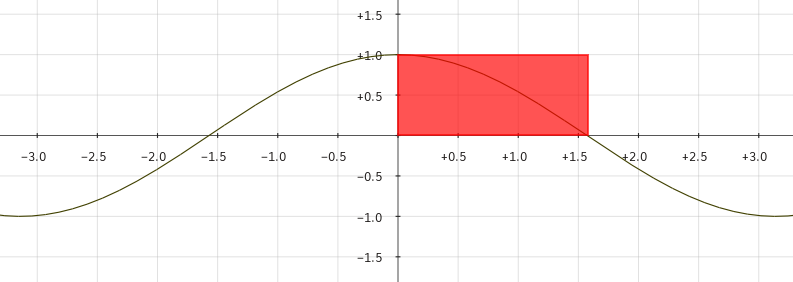
\includegraphics[width=0.8\textwidth]{img/coseno.png}
\caption{Comportamiento de la función $\cos$. En rojo la región que pertenece a la función de similitud}
\label{bus:img-coseno}
\end{figure}

Dos vectores proporcionales tiene la misma dirección y el ángulo entre ellos es cero, entonces la función de similitud es 1. Lo que significa que esta medida de similitud no considera el peso de cada tópico, por lo tanto no diferencia entre un artículo profesional y un artículo de un diario que cubre el mismo tópico. Esta debilidad de la medida basada en el ángulo no interfiere en este trabajo por la segunda propiedad de los vectores del problema, porque para que dos vectores sean proporcionalmente iguales tienen que ser idénticos y en tal caso es correcto que la similitud entre ellos sea 1.\\
El cálculo de similitud de los artículos, autores y universidades se realizó previamente a la ejecución de los algoritmos de búsquedas. El motivo por el cual se decidió hacer de esta manera fue para simplificar la ejecución ya que el costo de calcular el $\cos(\theta)$ de los vectores es alto.
\section{Atracciones turísticas}
Se utilizó una instancia de datos correspondiente a 200 atracciones turísticas de Europa \cite{turisticAtraction}. Ésta contiene la información del valor de la visita, que tipo de atracción es (parque, museo, edificio) y la similitud existente entre ellas. En contraste a lo trabajado con los datos de la instancia anterior, el presupuesto no define de antemano la cantidad de elementos que contendrán los bundles sino que el mismo estará relacionado con el valor informado. La similitud entre los distintos elementos esta basada en la distancia geográfica que existe entre ellos. Como atributo para calcular la complementaridad se eligió el tipo de atracción turística a la que pertenece cada uno de los elementos.\\

Las búsquedas que se hicieron en este caso tienen como propósito mostrar al usuario circuitos turísticos que puede realizar por día (cada bundle se puede interpretar como día). Al utilizar la distancia como similitud se está poniendo énfasis en que el turista pueda recorrer las atracciones de una manera ordenado sin tener que trasladarse de un extremo a otro de la ciudad o país. Con la elección de la complementaridad el viajante va a estar seguro que sea cual fuera su elección nunca visitará por ejemplo dos museos en un mismo día. Como todo turista cuenta con un presupuesto estimado por día para su viaje y para gastar en las visitas que desea realizar. Como las restricciones del armado de cada conjunto está restringido por el presupuesto máximo que se ingresa al comenzar las búsquedas, el usuario sabe que ningún circuito excede el valor que él calculo debe gastar por día. Así mismo tiene conocimiento de que no todos los circuitos tendrán la misma cantidad de atracciones ya que dependerá exclusivamente del presupuesto previo.
